% !TeX encoding = UTF-8
% !TeX spellcheck = hu_HU
%----------------------------------------------------------------------------
\chapter{\bevezetes}
%----------------------------------------------------------------------------

%A bevezető tartalmazza a diplomaterv-kiírás elemzését, történelmi előzményeit, a feladat indokoltságát (a motiváció leírását), az eddigi megoldásokat, és ennek tükrében a hallgató megoldásának összefoglalását.
%
%A bevezető szokás szerint a diplomaterv felépítésével záródik, azaz annak rövid leírásával, hogy melyik fejezet mivel foglalkozik.

Napjainkban az informatika és az internet életünk szerves részévé vált. A számos szolgáltatás folyamatos rendelkezésre állásának biztosítása és a megnövekedett forgalom kiszolgálása jó néhány új technológia kifejlesztését követelte meg.

Dolgozatomban elsősorban egy általános képet szeretnék adni arról, hogy milyen üzemeltetési kihívásokkal kell szembenéznünk, ha egy ilyen szolgáltatás működtetésébe vágjuk a fejszénket. Értekezésemben nem fogok kitérni bizonyos infrastrukturális hátterekre -- mint például a kiszolgálók folyamatos energiaellátásának biztosítása --, ezeket adottnak fogom tekinteni, hiszen ezt egy adatközpontban bérelt hely esetén sem magunknak kell biztosítanunk. A következőkben sokkal inkább az informatikai lehetőségek tárgyalására fogom helyezni a hangsúlyt: hogyan tudunk hatékonyan üzemeltetni több kiszolgálót, milyen módon lehet biztosítani a szolgáltatásaink lehető legnagyobb rendelkezésre állását, és hogyan védhetjük meg adatainkat egy esetlegesen félresikerült rendszerfrissítést követően.

A dolgozatban érinteni fogom a jelenleg legelterjedtebb virtualizációs technológiákat, melyek főbb tulajdonságait röviden ismertetem, valamint össze is hasonlítom ezeket a megoldásokat a legfontosabb különbségekre kitérve.

Szerepet fog kapni továbbá a logikai kötetkezelés, ezen belül is a Linux kernelben elérhető LVM-implementáció. Ez a technológia nagyban megkönnyíti a háttértárak és partíciók kezelését üzemeltetési szempontból, melyet főként virtualizációt végző fizikai gépek esetében használhatunk ki, hiszen ilyen helyzetekben érdemes minden virtuális rendszernek külön partíciót létrehozni, amelyek kezelése (pl. egy esetleges bővítés során) a hagyományos particionálási megoldásokkal sokkal összetettebb feladat lenne.

Szót ejtek a monitoring megoldásokról is, melyek elengedhetetlenek ahhoz, hogy a rendszer üzemeltetését végző szakemberek pontos képet kapjanak az infrastruktúra aktuális állapotáról, az esetleges korábbi problémákról. A monitorozás azért is fontos, mert ha egy hibát ezáltal sikerül idejekorán felismerni (például háttértárak esetén egy megfelelő határék beállításával időben értesülhetünk egy partíció megteléséről, és nem csak az írási hibákat tapasztaljuk), akkor elkerülhetőek a további, komolyabb hibák, amik akár a felhasználók számára is fennakadásokat okozhatnak. Az általam létrehozott tesztkörnyezetben is bemutatok egy ilyen monitoring megoldást, melynek segítségével az általam létrehozott infrastruktúra gépeit fogom folyamatosan ellenőrizni.

A tesztkörnyezet beállításában nagy szerep fog jutni a választott konfigurációmenedzsment szoftvernek, a Salt-nak. Ez arra fog lehetőséget biztosítani, hogy egyes konfigurációs fájlokat egyszerűen telepíthessünk több számítógépre is, valamint a keretrendszer leírónyelvén meghatározott konfigurációleíró szoftver lehetővé teszi azt is, hogy ellenőrizzük egyes szolgáltatások (service) állapotát. Ez hasznunkra válhat például egy saját service-szel érkező program telepítését követően, hiszen így a leíróban megadhatjuk a telepítés paramétereit, majd ezt követően egyből ellenőrizhetjük is, hogy a telepítés után sikeresen elindult-e az újonnan telepített szoftver.


A dolgozatban tárgyalt koncepciókat egy kisebb volumenű tesztrendszeren keresztül fogom bemutatni. Ennek a rendszernek a célja nem egy teljes vállalati környezet bemutatása, hiszen ehhez nagy mennyiségű hardverre, jelentős mértékű hardveres és szoftveres erőforrásokra lenne szükség, amelyek üzembe helyezése, összehangolása túlmutat a dolgozat keretein.
Ehelyett sokkal inkább arra szeretnék rávilágítani, hogy milyen eszközök állnak rendelkezésre egy ilyen nagyszabású infrastruktúra sikeres üzemeltetésének elősegítéséhez. Gondoljunk csak arra, hogy egy 5-10 számítógépből álló rendszer esetén kivitelezhető, hogy a rendszergazdák egyesével telepítsék a havi frissítéseket, azonban egy több száz, vagy több ezer kiszolgálóból álló nagyvállalati környezetben nem lenne egy reális elvárás.

Az ilyen és ehhez hasonló kihívások megoldására fogok lehetőségeket mutatni \aref{chap:technologies}.~fejezetben. Szó lesz a gépek távoli kezeléséről, folyamatos karbantartásukról, automatikus biztonsági javításokról (patchek) való értesülésről, ezek telepítéséről. Tárgyalni fogom továbbá a rendszert alkotó eszközök monitorozását, metrikák gyűjtését is, továbbá szó lesz az egyre szélesebb körben elterjedő konténerizációs technológiákról, ezek használatáról vállalati környezetekben. Bemutatom azt is, hogy a megfelelő eszközökkel milyen gyorsan hozhatunk létre konténereket, és mennyire hatékonyan kezelhetjük őket akár egy böngészőből is.
Fontos megjegyezni, hogy az itt említett technológiák kisebb környezetekben is használhatóak, azonban néhány esetben az ilyen rendszerek használata kevesebb előnyt nyújt, mint amennyi munkát telepítésük és karbantartásuk igényel, így érdemes felmérni az informatikai rendszerrel szemben támasztott elvárásainkat, és ennek megfelelően dönteni a szükséges technológiai komponensekről.

\Aref{chap:testenv}.~fejezetben fogom ismertetni az általam készített tesztkörnyezetet, ennek felépítését, a tervezési döntéseket, komponenseit, valamint az ezzel kapcsolatos munkáim során felmerült nehézségeket, tapasztalatokat. Ebben a fejezetben a korábban tárgyalt technológiák közül általam választott megoldásokat 

\section{Nagyvállalati környezetek ismertetése}
A vállalatok egyre nagyobb hangsúlyt fektetnek az informatikai rendszereik fejlesztésére és karbantartására, üzemeltetésére. Az ezek által nyújtott szolgáltatások sok esetben jelentős könnyebbséget jelentenek egyes üzleti folyamatokban, és a megfelelően automatizált munkafolyamatok csökkentik az egyes munkavállalók által elvégzendő manuális feladatokat. Fontos tisztában lenni azonban azzal, hogy ezek a megoldások csak akkor működnek jól a mindennapi használat során, ha sikerül biztosítani a megfelelő rendelkezésre állást, tehát egy -- a vállalat munkavállalói által a munkához nélkülözhetetlen -- szolgáltatásnak munkaidőben folyamatosan elérhetőnek kell lennie. Előfordulhatnak olyan igények is, amik miatt bizonyos, a vállalat működésének szempontjából nélkülözhetetlen szolgáltatásoknak folyamatosan elérhetőnek kell lenniük, mert a működésük nem munkaidőhöz kötött (ilyen lehet például a szervezet weboldala, illetve levelezőszervere).  Emellett a fent említett informatikai rendszerek karbantartásának is sokszor észrevehetetlennek kell lennie, azaz egy esetleges frissítés nem hátráltathatja a munkavégzést és a rendelkezésre állást. Az ilyen helyzetek kezelésére számos megoldás jött létre, ezek közül néhányat ismertetni fogok a következő fejezetben.

Egy másik fontos szempont a nagyvállalati rendszerek üzemeltetése -- és általában informatikai megoldások üzemeltetése és használata során -- ami napjainkban egyre nagyobb figyelmet kap, az IT-biztonság kérdése. A rendszerüzemeltetőknek tisztában kell lenniük a potenciális veszélyekkel, veszélyforrásokkal és fel kell készülniük egy esetleges támadásra, annak kezelésére. Sokszor hallhatunk a rendszeres biztonsági mentések fontosságáról, és ezek típusairól, követelményeiről. Egy jól bevett gyakorlat például az úgynevezett \textit{\mbox{3-2-1}}~mentési stratégia, ami egy jó kiindulási alapul szolgálhat minden szervezet számára a biztonsági mentésekhez.~\cite{Backblaze321}
A megoldás neve az alábbi elvekből származik:~\cite{Seagate321}
\begin{itemize}
	\item három példány az adatokról,
	\item két különböző eszközön (akár más típusú adathordozókon, pl. SSD, HDD, mágnesszalag -- ez segít az adathordozóra jellemző esetleges hibák hatásának csökkentésében),
	\item egy példányt földrajzilag különböző helyen tároljunk (pl. a cég székhelyén legyenek az eredeti adatok és még egy mentés, és egy példányt pedig tároljunk adatközpontban, vagy vegyünk igénybe harmadik féltől biztonságimentés-szolgáltatást).
\end{itemize}

A biztonsági mentések elvégzésére és automatizálására többféle megoldást választhat a szervezet az igényeihez igazodva. Bevett szokás például, hogy a cégen belüli mentéseket valamilyen mentést támogató vagy akár teljesen automatizáló szoftverrel oldják meg (például Bareos, Bacula, BackupPC). Az ilyen megoldások üzembe helyezése nehezebb lehet, mintha például csak egyéni scriptekkel hajtanánk végre a mentéseket, de hosszabb távon mégis célszerű lehet megfelelően konfigurálni őket, mert könnyebben kezelhetővé teszik egy komplex infrastruktúrában található gépek adatainak mentését, illetve az egyszer megírt konfigurációs fájlok több gépen is felhasználhatóak. Mindezek mellett ezek a szoftverek általában rendelkeznek valamilyen grafikus felhasználói felülettel (pl. webes interfész), amely tovább egyszerűsíti a mentések készítését, valamint szükség esetén a mentés visszaállítását.

% TODO: Bareos web UI kép lecserélése
\begin{figure}[!ht]
	\centering
	\includegraphics[width=150mm, keepaspectratio]{figures/bareos-dashboard.png}
	\caption{A Bareos biztonsági mentéseket végző program webes felületének részlete. Forrás: \url{https://www.bareos.com/bareos-webui-modules/}}
	\label{fig:bareos}
\end{figure}

Nagyvállalati környezetben nem hagyhatjuk ki a RAID-megoldásokat (a népszerű RAID 1 és RAID 6 megoldásokat \az{\ref{fig:raid} ábra} szemlélteti), ha szerverek biztonsági mentéséről beszélünk. Ezek arra adnak lehetőséget, hogy az adatokat több háttértáron (pl. merevlemez vagy SSD) tároljuk úgy, hogy egy esetleges diszk hiba ne okozzon fennakadást a működésben. Fontos tisztában lenni azonban azzal, hogy a RAID-megoldások nem védenek bizonyos veszélyek ellen (például zsarolóvírusok), hiszen az adatok duplikálása valós időben történik, így egy esetleges támadás során a RAID pool-ba bevont összes diszken megváltoznak az adatok, így nem alkalmas a támadás utáni visszaállításra. Emiatt egy RAID pool a \textit{3-2-1} mentési stratégiát alkalmazva csak egyetlen eszköznek tekinthető, hiába több lemezt használunk a mentés során. RAID-elést tehát csak hardveres hibák ellen érdemes használnunk, rosszindulatú támadás esetén ezek nem nyújtanak védelmet az adataink számára.

% TODO: RAID ábra, hivatkozások
\begin{figure}[!ht]
%	\centering
%	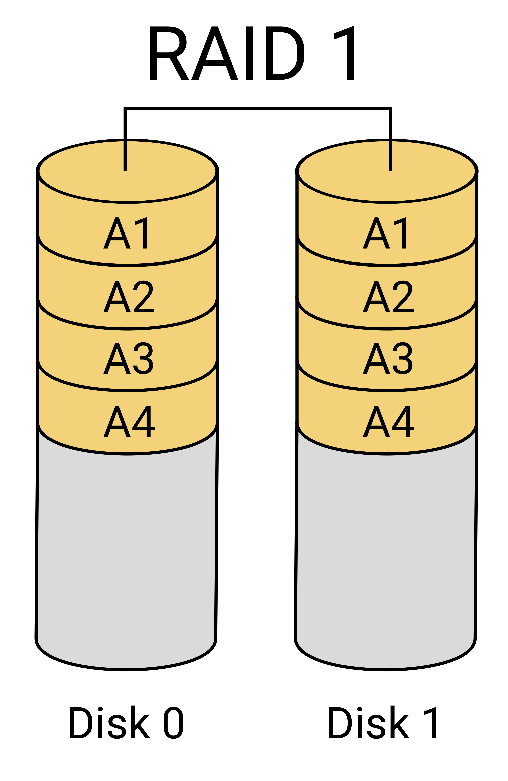
\includegraphics[height=70mm, keepaspectratio]{figures/raid1.pdf}
	
	\centering
	\begin{subfigure}{0.3\textwidth}
		\centering
		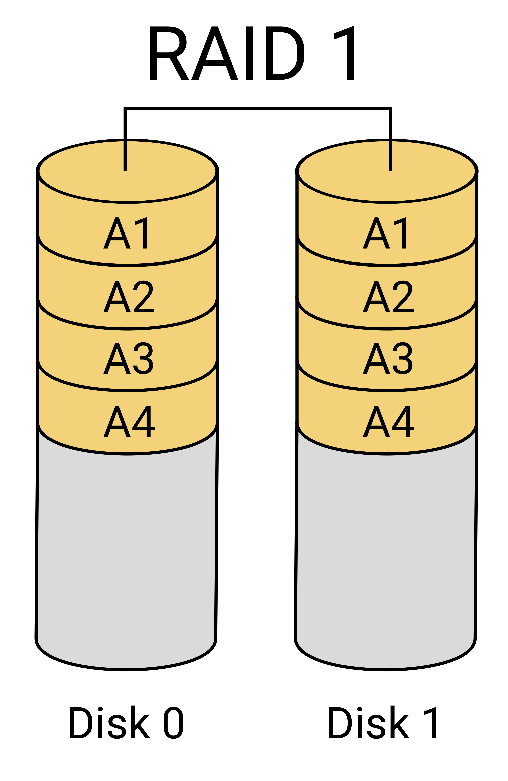
\includegraphics[keepaspectratio, height=52mm]{figures/raid1.pdf}
	\end{subfigure}
	\hspace{0.05\textwidth}
	\begin{subfigure}{0.6\textwidth}
		\centering
		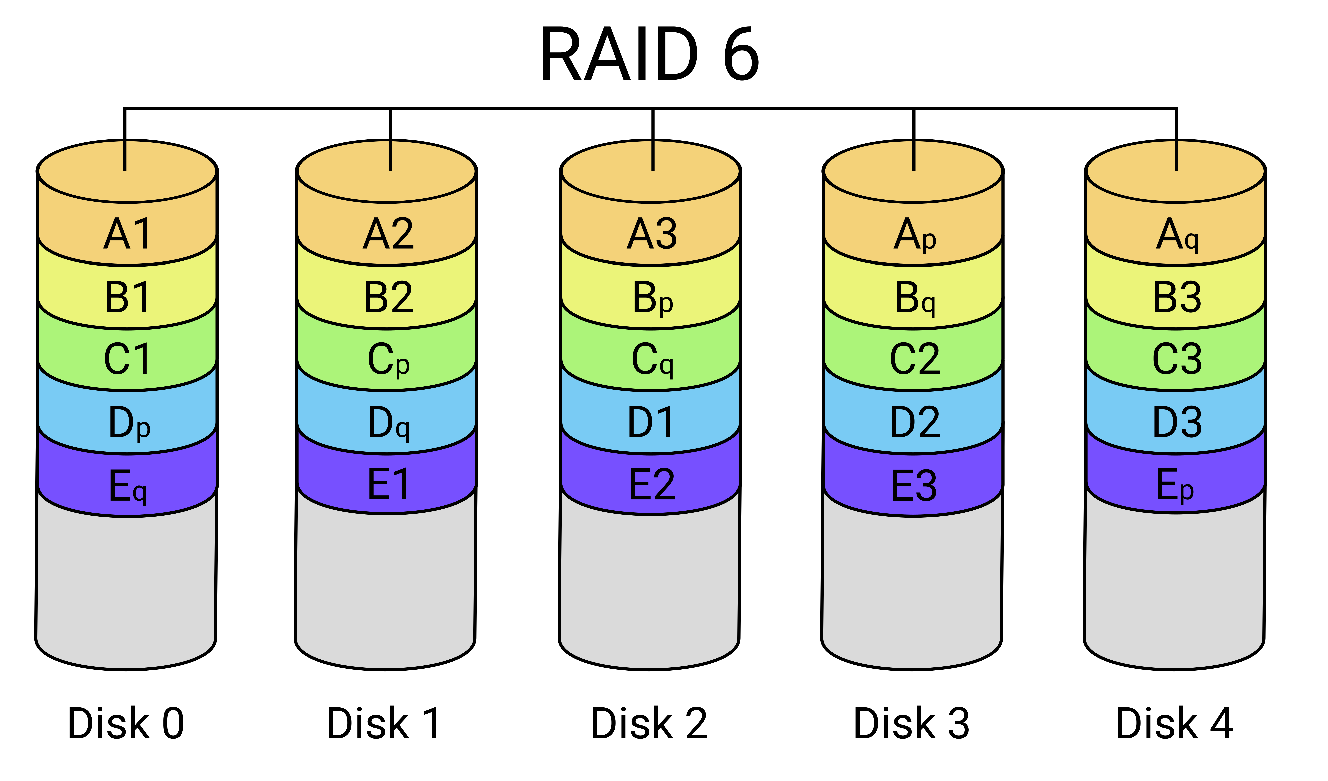
\includegraphics[keepaspectratio, height=52mm]{figures/raid6.pdf}
	\end{subfigure}
	\caption{RAID 1 és RAID 6 megoldások felépítése \cite{WikiRaidLevels}}
	\label{fig:raid}
\end{figure}

%\begin{figure}[h]
%	\centering
%	\begin{subfigure}{0.4\textwidth}
%		\centering
%		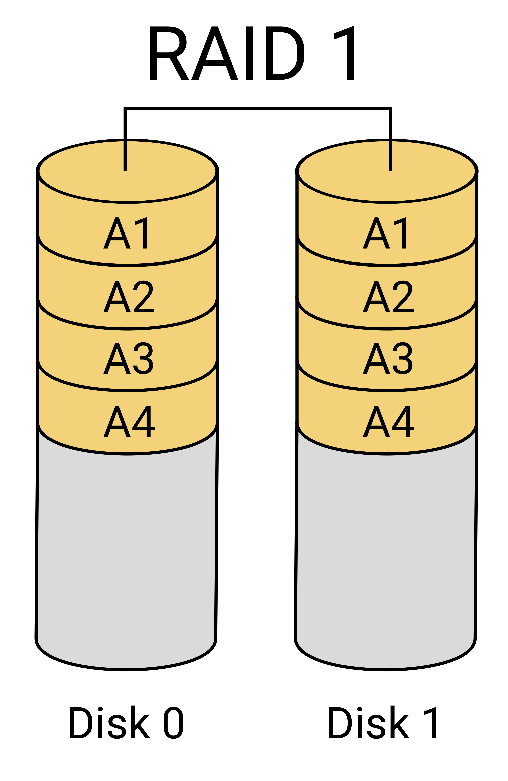
\includegraphics[keepaspectratio, scale=0.18]{figures/raid1}
%	\end{subfigure}
%	\hspace{0.075\textwidth}
%	\begin{subfigure}{0.3\textwidth}
%		\centering
%		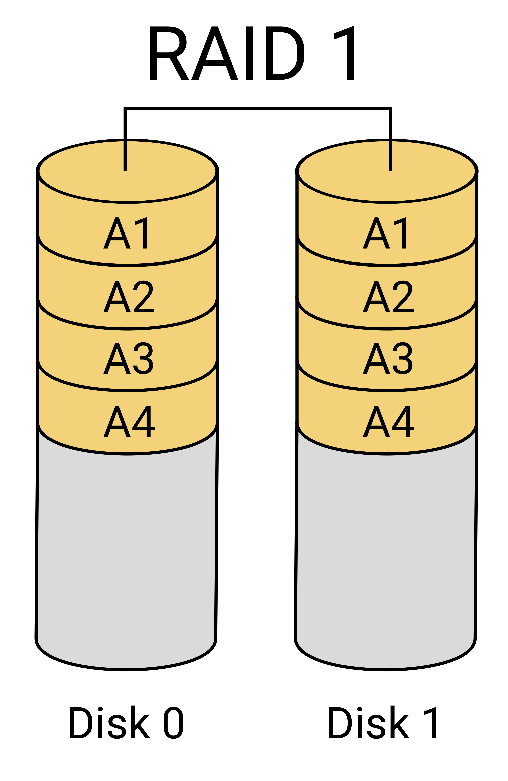
\includegraphics[keepaspectratio, scale=0.11]{figures/raid1}
%	\end{subfigure}
%	\caption{A Qt és a GTK logója}
%	\label{fig:qtgtklogo}
%\end{figure}

A legtöbb hétköznapi felhasználó számára ismeretlen vagy meglepő lehet, hogy maga az internet és az ezen keresztül elérhető szolgáltatások -- gondoljunk például az Ügyfélkapura vagy az internetbank-szolgáltatásokra -- nagyon komplex rendszerek nem csak szoftveres, hanem informatikai infrastruktúra szempontjából is. A legtöbb ilyen szolgáltatás egy adatközpontban lévő szerveren fut, ami a beérkező kérésekre ad válaszokat. Ezt a folyamatot úgy is felfoghatjuk, hogy az ilyen szolgáltatások felhasználói lényegében az adott szolgáltató (a fenti példánál maradva a Magyar Állam és az adott bankok) számítógépeivel kommunikálnak.

Ezek a szervergépek több lényeges különbséggel is bírnak a személyi számítógépekkel szemben. Egyik legfontosabb tulajdonságuk, hogy hibatűrőek bizonyos hardverhibákat illetően: szinte minden főbb komponensből legalább kettő áll rendelkezésre, így ha az egyik meg is hibásodik, akkor a hiba elhárításáig a beépített redundancia miatt a gép képes tovább funkcionálni, általában a felhasználók felé észrevétlenül, míg a gép üzemeltetői figyelmeztetést kapnak a hiba típusáról és a kapcsolódó tennivalókról.
% TODO: kép redundáns dolgokról (pl. hálózati kártya, PSU), és hibajelző elemekről (pl. CPU fault, RAM-hiba, diszk hiba)

\section{Virtualizáció}
A fent említett megnövekedett forgalom kiszolgálását hatékonyan lehet kezelni úgy, hogy olyan fizikai számítógépet helyezünk üzembe, mely  több, egymástól független operációs rendszer futtatására is alkalmas. Ilyenkor ezeket a fizikai gépen futó rendszereket virtuális gépeknek (virtual machine, VM) % TODO: rövidítésjegyzékbe
nevezzük. Egy virtuális gép elkülönített erőforrásokat kap a fizikai géptől, hozzáférhet például bizonyos mennyiségű processzormaghoz, memóriához, illetve külön háttértár-partíciói is lehetnek. A virtualizált hardverek és operációs rendszerek a legtöbb esetben a külvilág felé nem különböztethetőek meg a fizikai számítógépektől, és ezzel a megoldással jelentősen csökkenthető a rendszerek és a hozzájuk szükséges informatikai infrastruktúra üzemeltetésének költsége.

A virtualizáció nagy ereje abban rejlik, hogy bizonyos hardverek virtualizációjával egységnyi teljesítményt olcsóbban kaphatunk meg, mintha külön fizikai gépeket helyeznénk üzembe, illetve nagyobb rugalmasságot kapunk a kezelésükben, üzemeltetésükben. Képzeljük el, hogy megveszünk egy számítógépet, amin szeretnénk futtatni egy számunkra fontos alkalmazást, mondjuk a honlapunkat. Ilyenkor az ezen a gépen futó operációs rendszer teljes mértékben megszabhatja, hogy milyen erőforrásokból mennyit használ. Ha egy másik szolgáltatást -- például levelezőszervert -- szeretnénk emellett futtatni, akkor limitáltabbak a lehetőségeink, hiszen a korábban telepített webszerver már foglal bizonyos erőforrásokat, illetve a program függőségeit és konfigurációs fájljait is telepítettük már, ami esetleg negatívan hat a levelezőszerverünk működésére. Ha mindezt virtualizált környezetben tesszük meg, akkor a topológia megváltozik: a két alkalmazás teljesen elkülönítetten, egymás zavarása nélkül, különböző virtuális gépekben futhatnak, míg magán a fizikai gépen egy úgynevezett hypervisor látja el az erőforrások ütemezésének és kiosztásának (pl. processzoridő, memória) feladatát.
% TODO: virt-manager screenshot, esetleg virsh xml screenshot

\subsection{Népszerű virtualizációs technológiák}
Mivel a virtualizáció napjainkban nagyon elterjedt technológia, számos olyan megoldás született, mely egyszerűsíti a virtuális gépek üzemeltetését. Ezek közül nagy ismertségnek örvend az Oracle VirtualBox és a VMware Player, azonban ezek a megoldások nem skálázódnak annyira jól, mint a továbbiakban tárgyalt társaik, melyek sokkal megfelelőbbek nagyvállalati szerverkörnyezetben való alkalmazásra. Ezek a megoldások lehetőséget biztosítanak a virtuális gépek távoli elérésre, kezelésére, egyszerűbb telepítésükre, valamint szükség esetén elosztott működésükre.

Ilyen nagyvállalati környezetben is kedvelt megoldás például a VMware ESXi, amely egy igen modern hypervisor számos kényelmi funkcióval ellátva (lehetőség van például a rendszer webes felületről való kezelésére és virtuális gépek sablonból való gyors (nagyságrendileg 5-10 perc) telepítésére).
Egy másik kedvelt megoldás az ESXi-vel ellentétben teljesen ingyenesen, GPLv2-es licenc alatt elérhető XEN hypervisor, mely ugyan kevesebb kényelmi funkciót tartalmaz, de szintén népszerűségnek örvend széleskörű támogatása, kedvező teljesítménye és szabad szoftver voltából eredő ingyenessége miatt. A XEN a 2014 márciusában kiadott 4.4-es verzió óta stabilan működik együtt a libvirt virtualizációs API-val, amely nagyban megkönnyíti a hypervisorral való kommunikációt a virtuális gépek konfigurálása során.~\cite{Xen44ReleaseNotes}
% TODO: API, KVM rövidítésjegyzékbe
A XEN-hez hasonlóan szabad szoftver licenccel érhető el a Kernel-based Virtual Machine (KVM) is, mely a XEN-nél modernebb megoldásnak tekinthető, és manapság széles körben használják a Linux kernelbe való integráltságának és stabilitásának köszönhetően. Bár maga a KVM nem tartalmaz ilyet, de számos interfész elérhető az ezen keresztül futtatott virtuális gépek kezelésére (például virt-manager), valamint akadnak olyan megoldások is, melyek a KVM-re alapozva nyújtanak szélesebb körű virtualizációs megoldást, ilyen lehet\footnote{A konfigurációtól függően akár többfajta virtualizációs környezet is beállítható, de a KVM az egyik legjobban támogatott.} például a Proxmox és a Cockpit.


\subsection{Virtuális gépek használatának néhány előnye}
A virtualizáció számos előnnyel bír a szerverinfrastruktúra karbantartása, könnyű kezelhetősége szempontjából, ebből néhány fontosabbat szeretnék kiemelni.

\subsubsection{Erőforrások testreszabása}
Amikor több tíz vagy több száz szerver üzemeltetéséről van szó, akkor hatványozottan számításba kell vennünk az egyes gépekre jutó költségeket. Virtuális gépek esetén ez azért kedvezőbb egy fizikai gépnél, mert ugyan a nagyvállalati környezetbe szánt szervergépek jelentősen drágábbak a személyes felhasználásra tervezett társaiknál, de akár több tíz virtuális gép egyidejű futtatását is lehetővé teszik. Ezáltal az egy fizikai gépre eső, asztali gépeknél megszokott áramfogyasztáshoz képest jóval nagyobb energiafelvétel sokkal kedvezőbb arányt mutat, ha számításba vesszük a futtatott virtuális kiszolgálók számát is.

Mindezek mellett a nagyvállalati felhasználáshoz tervezett számítógépek jóval hibatűrőbbek, hiszen a főbb komponensek redundánsan lettek kialakítva: ezekből az ilyen szerverekben legalább kettő van, és a rendszer automatikusan képes detektálni a hardveres hibákat, és ezek figyelembe vételével tovább működni. További előny lehet még hardveres hibák esetén, hogy ezek a számítógépek széles körben támogatják az úgynevezett \textit{hot swappingot}, amely azt jelenti, hogy bizonyos hardverelemek (általában például háttértárak és memóriamodulok) a számítógép bekapcsolt állapotában, annak működése közben is szolgáltatás nélkül cserélhetőek.

Előnyös lehet továbbá, hogy a virtuális gépek erőforrásai szabadon módosíthatók, így akár két újraindítás között is változtathatjuk a rendelkezésre álló memória mennyiségét vagy épp a processzormagok számát. Sőt, egyes hypervisorok és operációs rendszerek ezen erőforrások futásidejű megváltoztatását is támogatják bizonyos korlátozások mellett, így gyakorlatilag a fontosabb virtualizált erőforrások is hot swappelhetőnek tekinthetőek.

\subsubsection{Snapshotok}
Egy másik kedvező lehetőség virtuális gépek használata esetén az, hogy úgynevezett snapshotokat készíthetünk róluk. Ezek a snapshotok a gépet egy adott pillanatbeli állapotban reprezentálják, és később ezeket az állapotokat visszaállíthatjuk, ha szükségünk lesz rá. Egyes megoldások a memóriakép mentését is támogatják, így akár egy futó gép is könnyen visszaállítható. A snapshotok készítése hasznos lehet például rendszerfrissítések esetén, így ha valamiféle hiba lép fel a frissítés során, vagy egy adott szoftver nem megfelelően működik azt követően, akkor a frissítés előtt készített snapshotra visszaállva újra teljes értékűen üzemelhet a szerver, amíg a frissítés során fellépő hibát elhárítjuk.

\subsubsection{Migráció}
Részben az előző ponthoz kapcsolódik a virtuális gépek migrációja. Ez a funkció azt jelenti, hogy egy adott fizikai gépről, mely virtuális gépeket futtat (virtual host), készíthetünk egy snapshotot, amit áthelyezhetünk egy másik virtual hostra, és a virtuális gép ezen futhat tovább egyéb újrakonfigurálás nélkül.
Lehetőség van azonban a háttértárak tartalmát elhagyva is átmozgatni egy VM-et egy másik hosztra. Ehhez bevett szokás leírófájlok használata, mely egy virtuális gép konfigurációját tartalmazza. A leírófájlt egy másik hosztgépre áthelyezve ott újra elindíthatjuk a definiált virtuális gépet. Ilyenkor szükség lehet a VM háttértárainak inicializálására, de ettől eltekintve a konfiguráció szabadon hordozható virtual host-ok között. Ilyen migrációra egyes megoldások fejlettebb támogatást is adnak, így akár valós időben, az aktuális terheltség figyelembe vétele mellett automatikusan is áthelyezhetőek virtuális gépek a megadott fizikai hosztok között.
% TODO: listing egy példa virsh xml-lel

\subsection{Teljes virtualizáció és paravirtualizáció összehasonlítása}
\subsection{Konténerizáció}

\section{Logikai kötetkezelés}
\subsection{Snapshotok, mentések készítése}

